%%%%%%%%%%%%  Generated using docx2latex.com  %%%%%%%%%%%%%%

%%%%%%%%%%%%  v2.0.0-beta  %%%%%%%%%%%%%%

% This template is made using Docx2Latex add-on for Google
% Docs, Refer following videos 
% Getting started : 
% 
% How to use add on :
% 
\documentclass[12pt]{article}

 %%%%%%%%%%%%  Include Packages  %%%%%%%%%%%%%%


\usepackage{txfonts}
\usepackage{setspace}
\usepackage[a4paper,left=1.0in,right=1.0in,top=1.0in,bottom=1.0in,headheight=1in]{geometry}
\usepackage{fancyhdr}
\fancypagestyle{plain}{%
 \fancyhf{}
 \fancyfoot[CE]{Pune Institute of Computer Technology, Department of Computer Engineering 2017-18}
 \fancyfoot[RE]{\thepage}
}
\pagestyle{fancy}
\fancyhead{}
\renewcommand{\headrulewidth}{0pt}
\footskip = 0.625in
\cfoot{}
\rfoot{}
% removes the horizontal line in certificate
\setlength\arrayrulewidth{0pt}
% Blank space below is for aesthetics purpose only
\usepackage{amsmath}
\usepackage{latexsym}
\usepackage{amsfonts}
\usepackage[normalem]{ulem}
\usepackage{array}
\usepackage{amssymb}
\usepackage{graphicx}
\usepackage[backend=biber,
style=numeric,
sorting=none,
isbn=false,
doi=false,
url=false,
]{biblatex}\addbibresource{bibliography.bib}

\usepackage{subfig}
\usepackage{wrapfig}
\usepackage{wasysym}
\usepackage{enumitem}
\usepackage{adjustbox}
\usepackage{ragged2e}
\usepackage[svgnames,table]{xcolor}
\usepackage{tikz}
\usepackage{longtable}
\usepackage{changepage}
\usepackage{hhline}
\usepackage{multicol}
\usepackage{tabto}
\usepackage{float}
\usepackage{multirow}
\usepackage{makecell}
\usepackage[toc,page]{appendix}
\usepackage[hidelinks]{hyperref}
\usetikzlibrary{shapes.symbols,shapes.geometric,shadows,arrows.meta}
\tikzset{>={Latex[width=1.5mm,length=2mm]}}
\usepackage{flowchart}\usepackage[utf8]{inputenc}
\usepackage[T1]{fontenc}
\TabPositions{0.5in,1.0in,1.5in,2.0in,2.5in,3.0in,3.5in,4.0in,4.5in,5.0in,5.5in,6.0in,}

\urlstyle{same}


 %%%%%%%%%%%%  Set Depths for Sections  %%%%%%%%%%%%%%

% 1) Section
% 1.1) SubSection
% 1.1.1) SubSubSection
% 1.1.1.1) Paragraph
% 1.1.1.1.1) Subparagraph


\setcounter{tocdepth}{5}
\setcounter{secnumdepth}{5}


 %%%%%%%%%%%%  Set Depths for Nested Lists created by \begin{enumerate}  %%%%%%%%%%%%%%


\setlistdepth{9}
\renewlist{enumerate}{enumerate}{9}
		\setlist[enumerate,1]{label=\arabic*)}
		\setlist[enumerate,2]{label=\alph*)}
		\setlist[enumerate,3]{label=(\roman*)}
		\setlist[enumerate,4]{label=(\arabic*)}
		\setlist[enumerate,5]{label=(\Alph*)}
		\setlist[enumerate,6]{label=(\Roman*)}
		\setlist[enumerate,7]{label=\arabic*}
		\setlist[enumerate,8]{label=\alph*}
		\setlist[enumerate,9]{label=\roman*}

\renewlist{itemize}{itemize}{9}
		\setlist[itemize]{label=$\cdot$}
		\setlist[itemize,1]{label=\textbullet}
		\setlist[itemize,2]{label=$\circ$}
		\setlist[itemize,3]{label=$\ast$}
		\setlist[itemize,4]{label=$\dagger$}
		\setlist[itemize,5]{label=$\triangleright$}
		\setlist[itemize,6]{label=$\bigstar$}
		\setlist[itemize,7]{label=$\blacklozenge$}
		\setlist[itemize,8]{label=$\prime$}

\setlength{\topsep}{0pt}\setlength{\parindent}{0pt}

 %%%%%%%%%%%%  This sets linespacing (verticle gap between Lines) Default=1 %%%%%%%%%%%%%%


\renewcommand{\arraystretch}{1.3}


%%%%%%%%%%%%%%%%%%%% Document code starts here %%%%%%%%%%%%%%%%%%%%



\begin{document}

\vspace{\baselineskip}
\begin{Center}
{\fontsize{14pt}{16.8pt}\selectfont \textbf{PUNE INSTITUTE OF COMPUTER TECHNOLOGY,}\par}
\end{Center}\par

\begin{Center}
{\fontsize{14pt}{16.8pt}\selectfont \textbf{DHANKAWADI PUNE-43.}\par}
\end{Center}\par

\begin{Center}
{\fontsize{26pt}{31.2pt}\selectfont \textbf{\textit{A Seminar Report}}\par}
\end{Center}\par

\begin{Center}
\textbf{\textit{ }\ \ \ \  }{\fontsize{24pt}{28.8pt}\selectfont \textbf{\textit{\ On  }\  }\par}
\end{Center}\par

\begin{Center}
{\fontsize{16pt}{19.2pt}\selectfont \textbf{Stock Market Prediction}\par}
\end{Center}\par

\begin{Center}
{\fontsize{14pt}{16.8pt}\selectfont  \par}
\end{Center}\par

\begin{Center}
{\fontsize{14pt}{16.8pt}\selectfont SUBMITTED BY\par}
\end{Center}\par

\begin{Center}
{\fontsize{14pt}{16.8pt}\selectfont  \par}
\end{Center}\par

\begin{Center}
{\fontsize{16pt}{19.2pt}\selectfont \textbf{NAME: Anurag Gujarathi}\par}
\end{Center}\par

\begin{Center}
{\fontsize{16pt}{19.2pt}\selectfont \textbf{ROLL NO: 3134}\par}
\end{Center}\par

\begin{Center}
{\fontsize{16pt}{19.2pt}\selectfont \textbf{CLASS: TE-1}\par}
\end{Center}\par

\begin{Center}
{\fontsize{7pt}{8.4pt}\selectfont \textbf{ }\par}
\end{Center}\par

\begin{Center}
{\fontsize{14pt}{16.8pt}\selectfont GUIDED BY\par}
\end{Center}\par

\begin{Center}
{\fontsize{16pt}{19.2pt}\selectfont \textbf{PROF. A. G. Phakatkar}\par}
\end{Center}\par



%%%%%%%%%%%%%%%%%%%% Figure/Image No: 1 starts here %%%%%%%%%%%%%%%%%%%%

\begin{figure}[H]
	\begin{Center}
		
\includegraphics[width=1.57in,height=1.57in]{./media/image1.jpg}
	\end{Center}
\end{figure}


%%%%%%%%%%%%%%%%%%%% Figure/Image No: 1 Ends here %%%%%%%%%%%%%%%%%%%%

\tab \par

 \par

 \par

 \par

\begin{Center}
{\fontsize{20pt}{24.0pt}\selectfont \textbf{COMPUTER ENGINEERING DEPARTMENT}\par}
\end{Center}\par

\begin{Center}
{\fontsize{20pt}{24.0pt}\selectfont \textbf{Academic Year: 2018-19}\par}

 %%%%%%%%%%%%  Starting New Page here %%%%%%%%%%%%%%

\newpage

\end{Center}\par


\vspace{\baselineskip}
\begin{Center}
{\fontsize{20pt}{24.0pt}\selectfont \textbf{ }\par}
\end{Center}\par

\begin{Center}
{\fontsize{14pt}{16.8pt}\selectfont \textbf{PUNE INSTITUTE OF COMPUTER TECHNOLOGY,}\par}
\end{Center}\par

\begin{Center}
{\fontsize{14pt}{16.8pt}\selectfont \textbf{DHANKAWADI PUNE-43.}\par}
\end{Center}\par


\vspace{\baselineskip}
\begin{Center}
{\fontsize{26pt}{31.2pt}\selectfont \textbf{\textit{CERTIFICATE}}{\fontsize{14pt}{16.8pt}\selectfont  \par}\par}
\end{Center}\par



%%%%%%%%%%%%%%%%%%%% Figure/Image No: 2 starts here %%%%%%%%%%%%%%%%%%%%

\begin{figure}[H]
	\begin{Center}
		
\includegraphics[width=1.57in,height=1.57in]{./media/image1.jpg}
	\end{Center}
\end{figure}


%%%%%%%%%%%%%%%%%%%% Figure/Image No: 2 Ends here %%%%%%%%%%%%%%%%%%%%

\begin{Center}
{\fontsize{14pt}{16.8pt}\selectfont  \par}
\end{Center}\par

\begin{justify}
{\fontsize{18pt}{21.6pt}\selectfont This is to certify that {\fontsize{20pt}{24.0pt}\selectfont Mr.\textit{ \textbf{\uline{Anurag Gujarathi}}}{\fontsize{18pt}{21.6pt}\selectfont \textit{, R}oll No\textbf{. }{\fontsize{20pt}{24.0pt}\selectfont \textbf{\uline{3134}}{\fontsize{18pt}{21.6pt}\selectfont \uline{ }a student of T.E. (Computer Engineering Department) Batch 2016-2019, has satisfactorily completed a seminar report on $``${\fontsize{16pt}{19.2pt}\selectfont \textbf{Stock Market Prediction$"$ }{\fontsize{18pt}{21.6pt}\selectfont \  under the guidance of\par}\par}\par}\par}\par}\par}\par}
\end{justify}\par

\begin{justify}
{\fontsize{18pt}{21.6pt}\selectfont \uline{Prof. A. G. Phakatkar} towards the partial fulfillment of the third year Computer Engineering Semester II of Pune University.\par}
\end{justify}\par

\begin{justify}
{\fontsize{18pt}{21.6pt}\selectfont  \par}
\end{justify}\par


\vspace{\baselineskip}


%%%%%%%%%%%%%%%%%%%% Table No: 1 starts here %%%%%%%%%%%%%%%%%%%%


\begin{table}[H]
 			\centering
\begin{tabular}{p{2.94in}p{2.94in}}
\hline
%row no:1
\multicolumn{1}{p{2.94in}}{Prof. A. G. Phakatkar } & 
\multicolumn{1}{p{2.94in}}{\Centering Dr.\ R.B.Ingle  } \\
\hhline{~~}
%row no:2
\multicolumn{1}{p{2.94in}}{\textbf{Internal Guide}\textit{\  }} & 
\multicolumn{1}{p{2.94in}}{\Centering \textbf{Head of Department\textit{,}}} \\
\hhline{~~}
%row no:3
\multicolumn{1}{p{2.94in}}{} & 
\multicolumn{1}{p{2.94in}}{\Centering \textbf{Computer Engineering} } \\
\hhline{~~}

\end{tabular}
 \end{table}


%%%%%%%%%%%%%%%%%%%% Table No: 1 ends here %%%%%%%%%%%%%%%%%%%%


\vspace{\baselineskip}
\setlength{\parskip}{6.0pt}
{\fontsize{14pt}{16.8pt}\selectfont \textbf{Date:}\par}\par

{\fontsize{14pt}{16.8pt}\selectfont \textbf{Place:}\par}

 %%%%%%%%%%%%  Starting New Page here %%%%%%%%%%%%%%

\newpage
\par

 \par


\vspace{\baselineskip}
{\fontsize{14pt}{16.8pt}\selectfont \textbf{\textit{Abstract:}}\par}\par

\begin{justify}
\textit{\textcolor[HTML]{000009}{A stock market is the aggregation of buyers and sellers which represent ownership claims on businesses. Intelligent investments in the stock market can potentially earn high returns to investors. However, due to the non-linear nature of stock market fluctuations, it is difficult to make an intelligent decision. This leads to the need of a model, which can predict the stock market on the basis of historical data. Concepts like Regression, Artificial Neural Networks and Support Vector Machines make it possible to predict values on the basis of historical data. A model for estimating the daily opening and closing prices of the stock market has been proposed.}}
\end{justify}\par

\begin{justify}
{\fontsize{14pt}{16.8pt}\selectfont \textbf{\textit{ }}\par}
\end{justify}\par

\begin{justify}
{\fontsize{14pt}{16.8pt}\selectfont \textbf{\textit{Keywords}}\textit{:} \textit{\textcolor[HTML]{00000A}{Stock market prediction, Regression, Neural Networks, Support Vector Machine}}\par}
\end{justify}\par

\begin{justify}
\textit{\textcolor[HTML]{00000A}{ }}

 %%%%%%%%%%%%  Starting New Page here %%%%%%%%%%%%%%

\newpage


 %%%%%%%%%%%%  Starting New Page here %%%%%%%%%%%%%%

\newpage

\end{justify}\par

\begin{Center}
{\fontsize{14pt}{16.8pt}\selectfont \textbf{ }\par}
\end{Center}\par

\begin{Center}
{\fontsize{16pt}{19.2pt}\selectfont \textbf{Prediction of Stock Market using historical data}\par}
\end{Center}\par

\begin{Center}
{\fontsize{14pt}{16.8pt}\selectfont \textbf{ }\par}
\end{Center}\par

 \par


% Following code generates Table Of Contents
% List Of Figures
% and Table Of Tables
\tableofcontents
\listoffigures
\listoftables
\newpage
\setlength\arrayrulewidth{0.4pt}
\renewcommand{\headrulewidth}{0.4pt}

\vspace{\baselineskip}

\vspace{\baselineskip}

\frontmatter
\chead{Seminar Title in the Header}
\rhead{\thepage}
\rfoot{``Department of Computer Engineering, PICT Pune” \ \ \ \ \ P:F/SMR-UG/08/R0}
\linespread{1.25}
\begin{justify}
 
\end{justify}\par

\section*{1\hspace*{10pt}Introduction }
\addcontentsline{toc}{section}{1\hspace*{10pt}Introduction }
\begin{justify}
The stock market is an aggregation of buyers and sellers of stocks, which represent ownership claims on businesses. Shares of stocks, equities and other securities of publicly listed companies can be traded on the Stock Exchange. An individual investor can participate in the trade of stocks on a Stock Exchange. The primary motive of an investor trading in the stock exchange is profitability.
\end{justify}\par

\begin{justify}
The stock market is volatile in nature. The price of a stock of a particular company may undergo multiple fluctuations within a day. An investor in the hope of making profit from the investment always looks towards an intelligent and well informed decision. It is difficult to gauge projected prices of a stock in future. Machine learning techniques are being utilized to predict the future prices of stocks.
\end{justify}\par

\begin{justify}
A predictive model which uses polynomial regression and support vector regression has been proposed to forecast prices of stocks on the basis of historical data. The patterns of fluctuations in historical data are recognized and future predictions are projected in accordance with these patterns. The stock prices data of technology companies like Google and Microsoft has been used in this prediction model.
\end{justify}\par


\vspace{\baselineskip}
\subsection*{1.1\hspace*{10pt}Motivation}
\addcontentsline{toc}{subsection}{1.1\hspace*{10pt}Motivation}
\begin{justify}
\ The stock market is known for providing a high return on investments. Intelligently designed and well executed decisions have the potential to earn exceptional profit. Many successful  investors have become billionaires with the stock market being their sole source of income. For example, Mr Warren Buffett. Conversely, poorly thought investment decisions can also lead to financial losses. Many unsuccessful investors have faced bankruptcy owing to the financial losses sustained while trading in the stock market.
\end{justify}\par

\begin{justify}
The stock market undergoes fluctuations routinely over the course of a day. The non-linear nature of these fluctuations makes it difficult to forecast the future prices of stocks at the time of investments. The quantification of an intelligent decision can be made after the return on investments is earned. Thus, a prediction model, which predicts future prices of a stock can aid in making an informed investment decision. Considering the prediction made by the model, an investor can judge the probability of profit and invest accordingly. Machine learning techniques like polynomial regression and support vector regression have been used.
\end{justify}\par


\vspace{\baselineskip}
\subsection*{1.2\hspace*{10pt}Literature Survey:}
\addcontentsline{toc}{subsection}{1.2\hspace*{10pt}Literature Survey:}
\subsubsection*{1.2.1\hspace*{10pt}Regression}
\addcontentsline{toc}{subsubsection}{1.2.1\hspace*{10pt}Regression}
\begin{justify}
[1] paper discusses the usage of regression algorithms in prediction of stock market. Support vector machines have a number of applications in prediction as mentioned in the paper. It also gives an overview of the shortcomings of support vector regression and the subsequent need to use particle swarm optimization. It was published in IEEE transactions on neural networks and learning systems.
\end{justify}\par


\vspace{\baselineskip}

\vspace{\baselineskip}
\subsubsection*{1.2.2\hspace*{10pt}Particle Swarm Optimization }
\addcontentsline{toc}{subsubsection}{1.2.2\hspace*{10pt}Particle Swarm Optimization }
\begin{justify}
[1] applies particle swarm optimization to a support vector regression model to increase the accuracy of prediction. Particle swarm optimization is a technique for iteratively selecting the best cost solution.
\end{justify}\par


\vspace{\baselineskip}

\vspace{\baselineskip}
\subsubsection*{1.2.3\hspace*{10pt}Deep Learning, Artificial Neural Networks}
\addcontentsline{toc}{subsubsection}{1.2.3\hspace*{10pt}Deep Learning, Artificial Neural Networks}
\begin{justify}
[2] was published in IEEE Access. It compares different techniques used to predict stock market prices. Deep learning, back propagation neural networks are some techniques that are discussed.
\end{justify}\par


\vspace{\baselineskip}

\vspace{\baselineskip}
\subsection*{1.3\hspace*{10pt}Challenges}
\addcontentsline{toc}{subsection}{1.3\hspace*{10pt}Challenges}
\begin{justify}
Being a non-linear model, finding a best fit curve exposes the algorithm to the problem of overfitting and underfitting. 
\end{justify}\par


\vspace{\baselineskip}
\subsubsection*{1.3.1\hspace*{10pt}Underfitting }
\addcontentsline{toc}{subsubsection}{1.3.1\hspace*{10pt}Underfitting }
\begin{justify}
Underfitting occurs when the model is unable to adequately capture the underlying structure of the data. It leads to a highly biased representation. Underfitting is typically observed when fitting a linear model to a non-linear data distribution. It leads to poor performance during prediction.
\end{justify}\par


\vspace{\baselineskip}
\subsubsection*{1.3.2\hspace*{10pt}Overfitting}
\addcontentsline{toc}{subsubsection}{1.3.2\hspace*{10pt}Overfitting}
\begin{justify}
Overfitting is observed when the predictive model is designed to fit the dataset too perfectly. In overfitting, some boundary line cases are also correctly classified or predicted. However, the downfall of this phenomenon is the increase in the degree of the polynomial representing the curve.
\end{justify}\par


\vspace{\baselineskip}

\vspace{\baselineskip}

\vspace{\baselineskip}


%%%%%%%%%%%%%%%%%%%% Figure/Image No: 3 starts here %%%%%%%%%%%%%%%%%%%%

\begin{figure}[H]
	\begin{Center}
		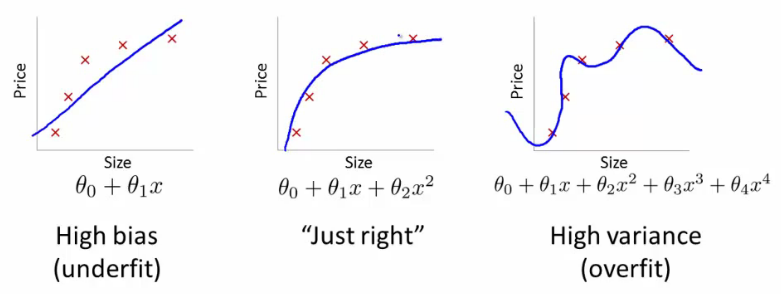
\includegraphics[width=6.27in,height=2.36in]{./media/image2.png}
	\end{Center}
\end{figure}


%%%%%%%%%%%%%%%%%%%% Figure/Image No: 3 Ends here %%%%%%%%%%%%%%%%%%%%

\par

\begin{adjustwidth}{0.5in}{0.0in}
\begin{Center}
\textbf{Figure 1. Underfitting and Overfitting}.
\end{Center}\par

\end{adjustwidth}


\vspace{\baselineskip}

\vspace{\baselineskip}
\setlength{\parskip}{12.0pt}
\section*{2\hspace*{10pt}Polynomial Regression}
\addcontentsline{toc}{section}{2\hspace*{10pt}Polynomial Regression}
\subsection*{2.1 Dataset}
\addcontentsline{toc}{subsection}{2.1 Dataset}
The dataset is obtained from Quandl API and accessed using Python’s Numpy array. The parameters of the dataset are Open, High, Low, Close, Volume, Adj. Open, Adj. High, Adj. Close, Adj. Low, Adj. Volume.\par


\vspace{\baselineskip}
In order to obtain the features of the dataset, following operations are performed.\par


\vspace{\baselineskip}


%%%%%%%%%%%%%%%%%%%% Figure/Image No: 4 starts here %%%%%%%%%%%%%%%%%%%%

\begin{figure}[H]
	\begin{Center}
		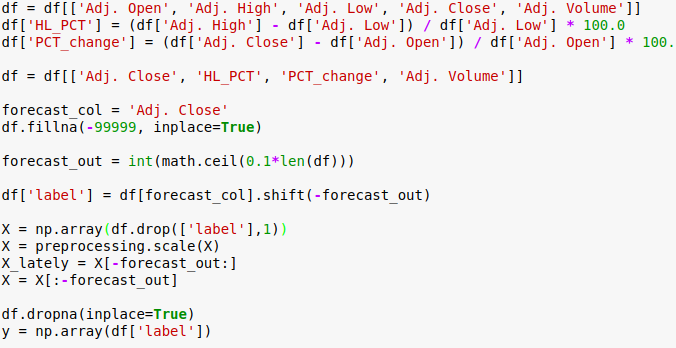
\includegraphics[width=6.27in,height=3.22in]{./media/image7.png}
	\end{Center}
\end{figure}


%%%%%%%%%%%%%%%%%%%% Figure/Image No: 4 Ends here %%%%%%%%%%%%%%%%%%%%

\par

\begin{Center}
\textbf{Figure 2. Obtaining features for regression}.
\end{Center}\par


\vspace{\baselineskip}
Following image represents the data obtained by the Quandl API.\par


\vspace{\baselineskip}


%%%%%%%%%%%%%%%%%%%% Figure/Image No: 5 starts here %%%%%%%%%%%%%%%%%%%%

\begin{figure}[H]
	\begin{Center}
		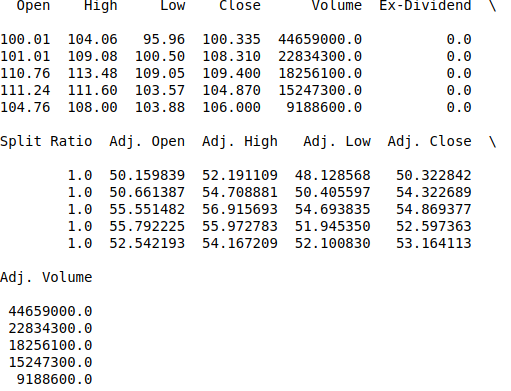
\includegraphics[width=5.32in,height=4.07in]{./media/image5.png}
	\end{Center}
\end{figure}


%%%%%%%%%%%%%%%%%%%% Figure/Image No: 5 Ends here %%%%%%%%%%%%%%%%%%%%

\par

\begin{Center}
\textbf{Figure 3. Parameters in the dataset.}
\end{Center}\par


\vspace{\baselineskip}

\vspace{\baselineskip}
\subsection*{2.2\hspace*{10pt}Features and Label}
\addcontentsline{toc}{subsection}{2.2\hspace*{10pt}Features and Label}

\vspace{\baselineskip}
Features obtained after manipulating raw data are Adj. Close, HL\_PCT, PCT\_Change, Adj. Volume. The objective of the regression model is to predict the closing stock prices. The forecast column of closing stock prices is shifted up by 10 percent of the size of the dataset and serves as the label for the regression model.\par

\subsection*{2.3\ \  \hspace*{10pt}Algorithm}
\addcontentsline{toc}{subsection}{2.3\ \  \hspace*{10pt}Algorithm}

\vspace{\baselineskip}
Following is the regression algorithm for prediction of closing stock prices of Google’s data. The library used for performing the prediction is scikit-learn. Pickle is the standard functionality provided by scikit-learn to load data into the model.\par



%%%%%%%%%%%%%%%%%%%% Figure/Image No: 6 starts here %%%%%%%%%%%%%%%%%%%%

\begin{figure}[H]
	\begin{Center}
		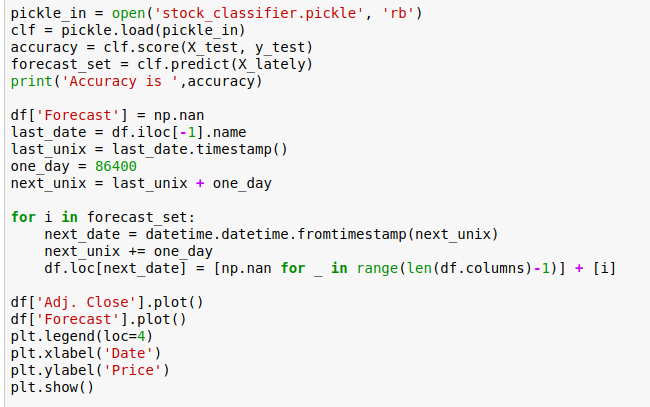
\includegraphics[width=6.27in,height=3.93in]{./media/image6.png}
	\end{Center}
\end{figure}


%%%%%%%%%%%%%%%%%%%% Figure/Image No: 6 Ends here %%%%%%%%%%%%%%%%%%%%

\begin{Center}
\\
\textbf{Figure 4. Code snippet of algorithm.}
\end{Center}\par


\vspace{\baselineskip}

\vspace{\baselineskip}
\subsection*{2.4 Result }
\addcontentsline{toc}{subsection}{2.4 Result }

\vspace{\baselineskip}
The last 10 percent of the dataset is forecasted by using the prediction model and compared with the values of the data. An accuracy of 70$\%$  is observed. Following graph depicts the result.\par


\vspace{\baselineskip}


%%%%%%%%%%%%%%%%%%%% Figure/Image No: 7 starts here %%%%%%%%%%%%%%%%%%%%

\begin{figure}[H]
	\begin{Center}
		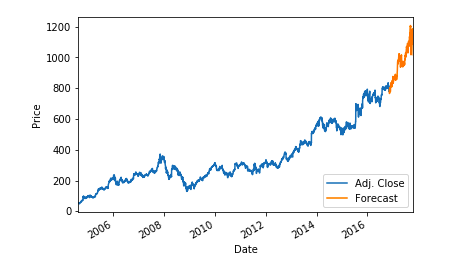
\includegraphics[width=4.88in,height=2.73in]{./media/image4.png}
	\end{Center}
\end{figure}


%%%%%%%%%%%%%%%%%%%% Figure/Image No: 7 Ends here %%%%%%%%%%%%%%%%%%%%

\par

\begin{Center}
\textbf{Figure 5. Result of prediction.}
\end{Center}\par

\section*{3\hspace*{10pt}Support Vector Regression.}
\addcontentsline{toc}{section}{3\hspace*{10pt}Support Vector Regression.}
\subsection*{3.1 Dataset}
\addcontentsline{toc}{subsection}{3.1 Dataset}

\vspace{\baselineskip}
Microsoft’s stock prices were used as the training data. This data was obtained from Kaggle. Following image represents the data.\par


\vspace{\baselineskip}


%%%%%%%%%%%%%%%%%%%% Figure/Image No: 8 starts here %%%%%%%%%%%%%%%%%%%%

\begin{figure}[H]
	\begin{Center}
		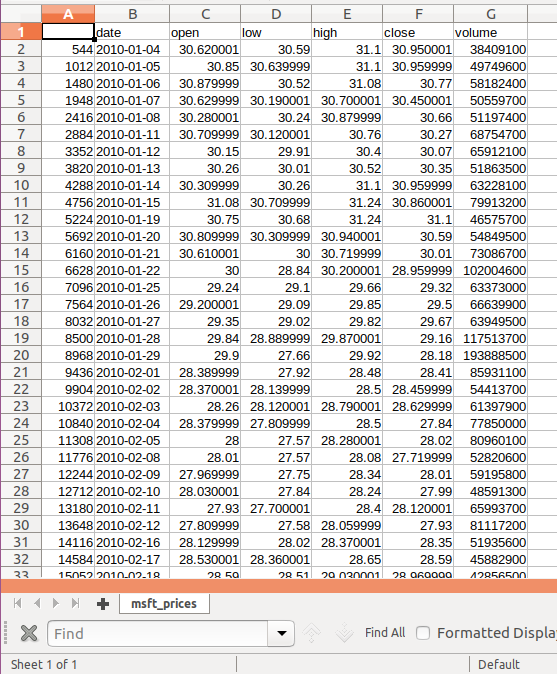
\includegraphics[width=5.8in,height=7.02in]{./media/image9.png}
	\end{Center}
\end{figure}


%%%%%%%%%%%%%%%%%%%% Figure/Image No: 8 Ends here %%%%%%%%%%%%%%%%%%%%

\par

\begin{Center}
\textbf{Figure 6. Microsoft’s dataset}
\end{Center}\par

\subsection*{3.2 Algorithm logic}
\addcontentsline{toc}{subsection}{3.2 Algorithm logic}

\vspace{\baselineskip}
Following code snippet gives the implementation of the support vector regression.\par


\vspace{\baselineskip}


%%%%%%%%%%%%%%%%%%%% Figure/Image No: 9 starts here %%%%%%%%%%%%%%%%%%%%

\begin{figure}[H]
	\begin{Center}
		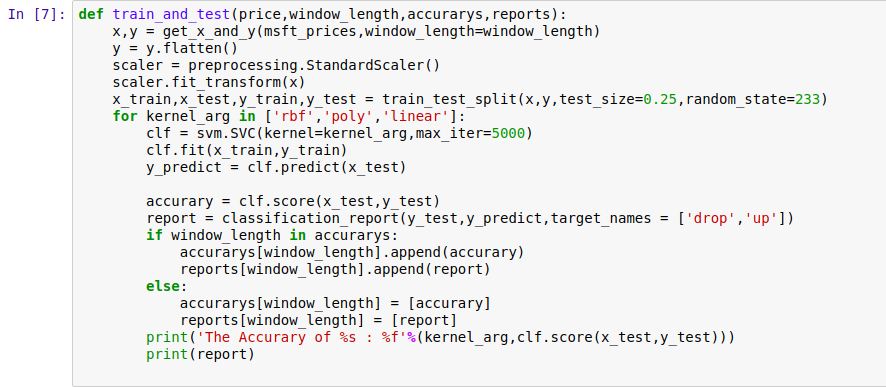
\includegraphics[width=6.97in,height=3.38in]{./media/image8.png}
	\end{Center}
\end{figure}


%%%%%%%%%%%%%%%%%%%% Figure/Image No: 9 Ends here %%%%%%%%%%%%%%%%%%%%

\par

\begin{Center}
\textbf{Figure 7. Code snippet of SVR} 
\end{Center}\par


\vspace{\baselineskip}

\vspace{\baselineskip}
\subsection*{3.3 Result}
\addcontentsline{toc}{subsection}{3.3 Result}

\vspace{\baselineskip}
3\ kernels - radial basis function, linear and polynomial were implemented.  Following is the result of the implementation.\par


\vspace{\baselineskip}


%%%%%%%%%%%%%%%%%%%% Figure/Image No: 10 starts here %%%%%%%%%%%%%%%%%%%%

\begin{figure}[H]
	\begin{Center}
		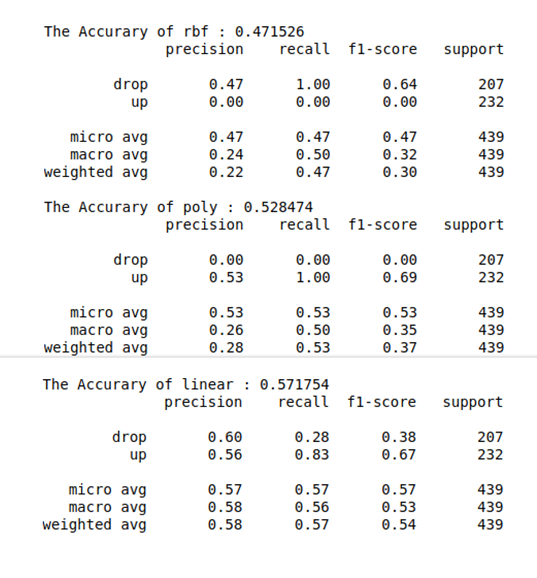
\includegraphics[width=5.59in,height=6.02in]{./media/image3.png}
	\end{Center}
\end{figure}


%%%%%%%%%%%%%%%%%%%% Figure/Image No: 10 Ends here %%%%%%%%%%%%%%%%%%%%

\par

\begin{Center}
\textbf{Figure 8. Result of support vector regression}
\end{Center}\par


\vspace{\baselineskip}
\section*{4\hspace*{10pt}Particle Swarm Optimization}
\addcontentsline{toc}{section}{4\hspace*{10pt}Particle Swarm Optimization}
In computational science, Particle Swarm Optimization (PSO) is a method that optimizes the problem by iteratively trying to improve a candidate solution with regard to a given measure of quality.\par

It solves a problem by having a population of candidate solutions, here called particles, and moving these particles around in the search space over the particle’s position and velocity.\par

\section*{5\hspace*{10pt}Conclusion and Future Enhancement}
\addcontentsline{toc}{section}{5\hspace*{10pt}Conclusion and Future Enhancement}
\subsection*{4.1\ \ \ \ \ \  Conclusion}
\addcontentsline{toc}{subsection}{4.1\ \ \ \ \ \  Conclusion}
\begin{enumerate}
	\item Using polynomial regression and support vector regression, accuracy of prediction model varies between 50$\%$  and 70$\%$  for the datasets used.\par

	\item The accuracy is dependent on training data.
\end{enumerate}\par

\subsection*{4.2\ \ \ \ \ \  Future Enhancements}
\addcontentsline{toc}{subsection}{4.2\ \ \ \ \ \  Future Enhancements}
\setlength{\parskip}{0.0pt}
\begin{itemize}
	\item Although stock prices can be predicted to a certain extent using only historic data, other factors also influence stock prices.\par

	\item Following factors also affect stock prices -\par

\begin{itemize}
	\item Economics\par

\begin{itemize}
	\item –Interest rates\par

	\item –Inflation\par


\end{itemize}
	\item Politics\par

\begin{itemize}
	\item –Government policy\par

	\item –Elections\par


\end{itemize}
	\item Natural and Man-made disasters\par

\begin{itemize}
	\item –Japan in 2011 tsunami\par

	\item –World War II\par


\end{itemize}
	\item Market Psychology\par

\begin{itemize}
	\item –Hype created by economists
\end{itemize}
\end{itemize}
\end{itemize}\par


\vspace{\baselineskip}
\begin{adjustwidth}{0.5in}{0.0in}
The predictive model must account for these factors in order to give a comprehensive prediction. These factors can be taken as input through a natural language classifier which processes current happenings through media reports.\par

\end{adjustwidth}

\setlength{\parskip}{12.0pt}
\begin{justify}
 
\end{justify}\par


\vspace{\baselineskip}
\setlength{\parskip}{9.96pt}

\begin{thebibliography}{99}

\vspace{\baselineskip}
\bibitem{item1}
Yongsheng Ding, Lijun Cheng, Witold Pedrycz and Kuangrong Hao, "Global Nonlinear Kernel Prediction for Large Data Set With a Particle Swarm-Optimized Interval Support Vector Regression" IEEE Transactions on Neural Networks and Learning Systems, Vol. 26, No. 10, October 2015\par

\bibitem{item2}
Chen, L., Qiao, Z., Wang, M., Wanga, C., Du, R., $\&$  Stanley, H. E. (2018). "Which artificial intelligence algorithm better predicts the Chinese stock market?" IEEE Access, 1–1.\par

\bibitem{item3}
\href{https://www.kaggle.com/rosand/fork-of-predict-stock-prices-with-svm}{\textit{\textcolor[HTML]{1155CC}{\uline{https://www.kaggle.com/rosand/fork-of-predict-stock-prices-with-svm}}}}\par


\vspace{\baselineskip}

\end{thebibliography}
\setlength{\parskip}{6.0pt}


 %%%%%%%%%%%%  Starting New Page here %%%%%%%%%%%%%%

\newpage

\vspace{\baselineskip}
\vspace{\baselineskip}
\begin{Center}
\textbf{\textsc{\uline{Appendix – D}}}
\end{Center}\par

\begin{Center}
{\fontsize{14pt}{16.8pt}\selectfont \textbf{\uline{Log Book }}\par}
\end{Center}\par

{\fontsize{14pt}{16.8pt}\selectfont \textbf{Roll No.\tab \tab \tab :- 3134}\par}\par

{\fontsize{14pt}{16.8pt}\selectfont \textbf{Name of the Student\tab :- Anurag Gujarathi}\par}\par

{\fontsize{14pt}{16.8pt}\selectfont \textbf{Name\ of\ the Guide   \tab :- Prof. A.G. Phakatkar}\par}\par

{\fontsize{14pt}{16.8pt}\selectfont \textbf{Seminar\ Title\   \tab \tab :- Stock Market Prediction}\par}\par


\vspace{\baselineskip}


%%%%%%%%%%%%%%%%%%%% Table No: 2 starts here %%%%%%%%%%%%%%%%%%%%


\begin{table}[H]
 			\centering
\begin{tabular}{p{0.56in}p{0.75in}p{2.31in}p{1.85in}}
\hline
%row no:1
\multicolumn{1}{|p{0.56in}}{\textbf{Sr. No.}} & 
\multicolumn{1}{|p{0.75in}}{\textbf{Date}} & 
\multicolumn{1}{|p{2.31in}}{\textbf{Details of Discussion/ Remarks}} & 
\multicolumn{1}{|p{1.85in}|}{\textbf{Signature of guide / Seminar Incharge}} \\
\hhline{----}
%row no:2
\multicolumn{1}{|p{0.56in}}{1.} & 
\multicolumn{1}{|p{0.75in}}{} & 
\multicolumn{1}{|p{2.31in}}{} & 
\multicolumn{1}{|p{1.85in}|}{} \\
\hhline{----}
%row no:3
\multicolumn{1}{|p{0.56in}}{2.} & 
\multicolumn{1}{|p{0.75in}}{} & 
\multicolumn{1}{|p{2.31in}}{} & 
\multicolumn{1}{|p{1.85in}|}{} \\
\hhline{----}
%row no:4
\multicolumn{1}{|p{0.56in}}{3.} & 
\multicolumn{1}{|p{0.75in}}{} & 
\multicolumn{1}{|p{2.31in}}{} & 
\multicolumn{1}{|p{1.85in}|}{} \\
\hhline{----}
%row no:5
\multicolumn{1}{|p{0.56in}}{4.} & 
\multicolumn{1}{|p{0.75in}}{} & 
\multicolumn{1}{|p{2.31in}}{} & 
\multicolumn{1}{|p{1.85in}|}{} \\
\hhline{----}
%row no:6
\multicolumn{1}{|p{0.56in}}{5.} & 
\multicolumn{1}{|p{0.75in}}{} & 
\multicolumn{1}{|p{2.31in}}{} & 
\multicolumn{1}{|p{1.85in}|}{} \\
\hhline{----}
%row no:7
\multicolumn{1}{|p{0.56in}}{6.} & 
\multicolumn{1}{|p{0.75in}}{} & 
\multicolumn{1}{|p{2.31in}}{} & 
\multicolumn{1}{|p{1.85in}|}{} \\
\hhline{----}
%row no:8
\multicolumn{1}{|p{0.56in}}{7.} & 
\multicolumn{1}{|p{0.75in}}{} & 
\multicolumn{1}{|p{2.31in}}{} & 
\multicolumn{1}{|p{1.85in}|}{} \\
\hhline{----}
%row no:9
\multicolumn{1}{|p{0.56in}}{8.} & 
\multicolumn{1}{|p{0.75in}}{} & 
\multicolumn{1}{|p{2.31in}}{} & 
\multicolumn{1}{|p{1.85in}|}{} \\
\hhline{----}
%row no:10
\multicolumn{1}{|p{0.56in}}{9.} & 
\multicolumn{1}{|p{0.75in}}{} & 
\multicolumn{1}{|p{2.31in}}{} & 
\multicolumn{1}{|p{1.85in}|}{} \\
\hhline{----}
%row no:11
\multicolumn{1}{|p{0.56in}}{10.} & 
\multicolumn{1}{|p{0.75in}}{} & 
\multicolumn{1}{|p{2.31in}}{} & 
\multicolumn{1}{|p{1.85in}|}{} \\
\hhline{----}

\end{tabular}
 \end{table}


%%%%%%%%%%%%%%%%%%%% Table No: 2 ends here %%%%%%%%%%%%%%%%%%%%

 \par

 \par


\vspace{\baselineskip}

\vspace{\baselineskip}
{\fontsize{14pt}{16.8pt}\selectfont \textbf{Student\ Signature\ \ \ \ \ \ \ \ \ \ \ \ \ \ \ \ \ \ \ \ \ \ \ \ \ \ \ \ \ \ \ \ \ \ \ \ \ \ \ \ \ \ \ \ \ \ \ \ \ \ \ \ \ \ \ \ \ \ \ \ \   Guide Signature}\par}\par

\begin{justify}
 
\end{justify}\par


\vspace{\baselineskip}

\printbibliography
\end{document}